%!TEX root = main.tex

\section{$L$-level Recommendation Policy}
In this section, we design an $L$-level recommendation policy for $L > 3$ and 2 arms. By having more than 3 levels, we get even smaller regret. 

Our recommendation policy has $L$ levels and two types of groups: $G$-groups and $\Gamma$-groups. Each level has $S^2$ $G$-groups for $S = 2^{10}\log(T)$. Label the $G$-groups in the $l$-th level as $G_{l,u,v}$ for $u,v \in [S]$. Level $2$ to level $L$ also have $S^2$ $\Gamma$-groups. Label the $\Gamma$-groups in the $l$-th level as $\Gamma_{l,u,v}$ for $u,v \in [S]$. 

We set the group size as following. For $l < L$,
\[
T_l = T^{\frac{2^{L-1} + 2^{L-2} + \cdots + 2^{L-l}}{2^{L-1}+ 2^{L-2} + \cdots + 1}}/S^3.
\]
and 
\[
T_L = (T - T_1 \cdot \GdT\cdot S^2 - (T_2 + \cdots + T_{l-1}) S^3) /S^3
\]
We restrict $L$ to be at most $\log(\ln(T)/\log(S^4))$ so that $T_l / T_{l-1} \geq T^{1/2^L} \geq S^4$ for $l = 2,...,L-1$. $T_L$ is a little bit different because we want total number of agents to be $T$. 
 
Each first-level group ($G_{1,u,v}$ for $u,v\in [S]$) has $T_1$ \ALGG of $\GdT$ rounds in parallel. For $l \geq 2$, there are $T_l$ agents in group $G_{l,u,v}$ and there are $T_l (S-1)$ agents in group $\Gamma_{l,u,v}$. 

Finally we define the information flow. Agents in the first level only observe the history defined in the \ALGG run. For agents in group $G_{l,u,v}$ with $l\geq 2$, they observe all the history in the first $l-2$ levels (both $G$-groups and $\Gamma$-groups) and history in group $G_{l-1,v,w}$ for all $w \in [S]$. Agents in group $\Gamma_{l,u,v}$ observe the same history as agents in group $G_{l,u,v}$.

\begin{figure}[H]
\centering
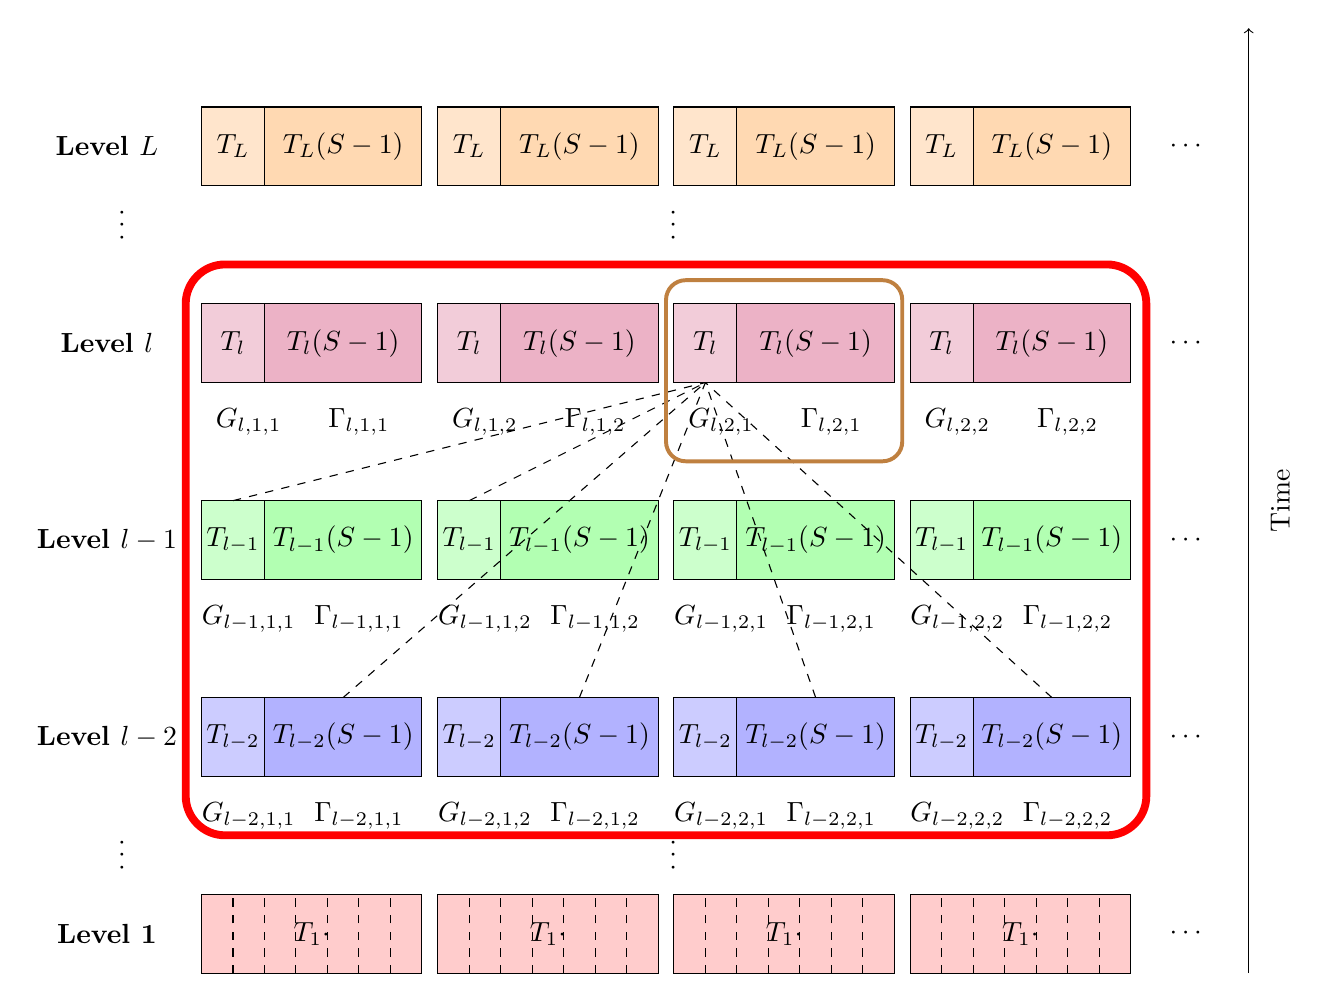
\begin{tikzpicture}  
 \foreach \x in {0,3,6,9}
 {
 \filldraw[fill=orange!20!white]
 (\x+0,10)--(\x+0.8,10)--(\x+0.8,11)--(\x+0,11)--cycle;
 \filldraw[fill=orange!30!white]
 (\x+0.8,10)--(\x+2.8,10)--(\x+2.8,11)--(\x+0.8,11)--cycle;
 \filldraw[fill=purple!20!white]
 (\x+0,7.5)--(\x+0.8,7.5)--(\x+0.8,8.5)--(\x+0,8.5)--cycle;
 \filldraw[fill=purple!30!white]
 (\x+0.8,7.5)--(\x+2.8,7.5)--(\x+2.8,8.5)--(\x+0.8,8.5)--cycle;
 \filldraw[fill=green!20!white]
 (\x+0,5)--(\x+0.8,5)--(\x+0.8,6)--(\x+0,6)--cycle;
 \filldraw[fill=green!30!white]
 (\x+0.8,5)--(\x+2.8,5)--(\x+2.8,6)--(\x+0.8,6)--cycle;
 \filldraw[fill=blue!20!white]
 (\x+0,2.5)--(\x+0.8,2.5)--(\x+0.8,3.5)--(\x+0,3.5)--cycle;
 \filldraw[fill=blue!30!white]
 (\x+0.8,2.5)--(\x+2.8,2.5)--(\x+2.8,3.5)--(\x+0.8,3.5)--cycle;
 \filldraw[fill=red!20!white]
 (\x+0,0)--(\x+2.8,0)--(\x+2.8,1)--(\x+0,1)--cycle;
 \draw[dashed] (\x+0.4,0)--(\x+0.4,1); 
 \draw[dashed] (\x+0.8,0)--(\x+0.8,1); 
 \draw[dashed] (\x+1.2,0)--(\x+1.2,1); 
 \draw[dashed] (\x+1.6,0)--(\x+1.6,1);  
 \draw[dashed] (\x+2,0)--(\x+2,1);  
 \draw[dashed] (\x+2.4,0)--(\x+2.4,1);  
 \node at(\x+0.4,3){$T_{l-2}$};
 \node at(\x+1.8,3){$T_{l-2} (S-1)$};
 \node at(\x+0.4,5.5){$T_{l-1}$};
 \node at(\x+1.8,5.5){$T_{l-1} (S-1)$};
 \node at(\x+0.4,8){$T_l$};
 \node at(\x+1.8,8){$T_l (S-1)$};
 \node at(\x+0.4,10.5){$T_L$};
 \node at(\x+1.8,10.5){$T_L (S-1)$};
 \node at(\x+1.4,0.5){$T_1 \cdot \GdT$};
 }
\foreach \y in {0,2.5,5,7.5,10}
{
  \node at (12.5,\y+0.5){$\cdots$};
} 
\foreach \u in {1,2}
{
	\foreach \v in {1,2}
	{
	\pgfmathsetmacro{\x}{((\u-1)*2+(\v-1))*3};
	\pgfmathsetmacro{\xa}{((\u-1))*3};
	\pgfmathsetmacro{\xb}{(2+(\u-1))*3};
   \node at(\x+0.6,7){$G_{l,\u,\v}$};
   \node at(\x+0.6,4.5){$G_{l-1,\u,\v}$};
   \node at(\x+0.6,2){$G_{l-2,\u,\v}$};
   \node at(\x+2,7){$\Gamma_{l,\u,\v}$};
   \node at(\x+2,4.5){$\Gamma_{l-1,\u,\v}$};
   \node at(\x+2,2){$\Gamma_{l-2,\u,\v}$};
   %\draw[dashed] (\x+0.4,3.5)--(\xa+0.4,5);  
   %\draw[dashed] (\x+0.4,3.5)--(\xb+0.4,5);  
   %\draw[dashed] (\x+0.4,3.5)--(\xa+1.8,5);  
   %\draw[dashed] (\x+0.4,3.5)--(\xb+1.8,5);  
   
   
   %\draw[dashed] (\x+0.4,6)--(\xa+0.4,7.5);  
   %\draw[dashed] (\x+0.4,6)--(\xb+0.4,7.5);  
   %\draw[dashed] (\x+0.4,6)--(\xa+1.8,7.5);  
   %\draw[dashed] (\x+0.4,6)--(\xb+1.8,7.5);  
	}
}

   \draw[dashed] (0+1.8,3.5)--(6.4,7.5);  	
   \draw[dashed] (3+1.8,3.5)--(6.4,7.5);  	
   \draw[dashed] (6+1.8,3.5)--(6.4,7.5);  	
   \draw[dashed] (9+1.8,3.5)--(6.4,7.5);  	
   
   %\draw[dashed] (0+0.4,3.5)--(6.4,7.5);  	
   %\draw[dashed] (3+0.4,3.5)--(6.4,7.5);  	
   %\draw[dashed] (6+0.4,3.5)--(6.4,7.5);  	
   %\draw[dashed] (9+0.4,3.5)--(6.4,7.5);  	
   
   \draw[dashed] (0+0.4,6)--(6.4,7.5);  	
   \draw[dashed] (3+0.4,6)--(6.4,7.5);  	
  \node at (6,1.5)[rotate = 90]{$\cdots$};
  \node at (-1,1.5)[rotate = 90]{$\cdots$};
  \node at (6,9.5)[rotate = 90]{$\cdots$};
  \node at (-1,9.5)[rotate = 90]{$\cdots$};
  \node at(-1.2,0.5){\textbf{Level 1}};
  \node at(-1.2,3){\textbf{Level $l-2$}};
  \node at(-1.2,5.5){\textbf{Level $l-1$}};
  \node at(-1.2,8){\textbf{Level $l$}};
  \node at(-1.2,10.5){\textbf{Level $L$}};
  \draw[->] (13.3,0)--(13.3,12);
  \node at(13.7,6)[ rotate=90]{Time};
  \draw [rounded corners=5mm, line width=1mm, red](-0.2,1.75)--(12,1.75)--(12,9)--(-0.2,9)--cycle;\draw [rounded corners=2.5mm, line width=0.5mm, brown](5.9,6.5)--(8.9,6.5)--(8.9,8.8)--(5.9,8.8)--cycle;
\end{tikzpicture}
\caption{$l$-level Recommendation Policy.}
\label{fig:llevel}
\end{figure}

\begin{theorem}
The $L$-level recommendation policy gets expected regret $O\left(T^{\frac{2^{L-1}}{2^L-1}} \log^2(T) \right)$ for $L \leq \log(\ln(T)/\log(10S^3))$. In particular, if we pick $L = \log(\ln(T)/\log(10S^3))$, the expected regret is at most $O(T^{1/2} \log^5(T))$. 
\end{theorem}

\begin{proof}
Wlog we assume $\mu_1 \geq \mu_2$ as the recommendation policy is symmetric to both arms. Similarly as the proof of Theorem \ref{thm:3level}, we start with some clean events.

\begin{itemize}
\item For $a \in \{1,2\}$, define $q_a$ to be the expected number of arm $a$ pulls in one run of \ALGG used in the first level. By Lemma \ref{lem:greedy}, we know $\GdP \leq q_a \leq \GdT$ For group $G_{1,u,v}$, define $W_1^{a,u,v}$ to be the event that the number of arm $a$ pulls in this group is between $q_a T_1- \GdT \sqrt{T_1\log(T)}$ and $q_a T_1 + \GdT \sqrt{T_1\log(T)}$. By Chernoff bound,
\[
\Pr[W_1^{a,u,v}] \geq 1-2\exp(-2\log(T)) \geq 1-2/T^2.
\]
Define $W_1$ to be the intersection of all these events (i.e. $W_1 = \bigcap_{a,u,v}W_1^{a,u,v}$). By union bound, we have
\[
\Pr[W_1] \geq 1- \frac{4S^2}{T^2}.
\]


\item For each agent $t$ and arm $a$, imagine there is a tape of enough arm $a$ pulls sampled before the recommendation policy starts and these samples are revealed one by one whenever agents in agent $t$'s observed history pull arm $a$.  Define $W_2^{t,a,t_1,t_2}$ to be the event that the mean of $t_1$-th to $t_2$-th pulls in the tape is at most $\sqrt{\frac{3\log(T)}{t_2-t_1+1}}$ away from $\mu_a$. By Chernoff bound, 
\[
\Pr[W_2^{t,a,t_1,t_2}] \geq 1 - 2\exp(-6\log(T)) \geq 1- 2/T^6.
\]

Define $W_2$ to be the intersection of all these events (i.e. $W_2 = \bigcap_{t,a,t_1,t_2} W_2^{t,a,t_1,t_2}$). By union bound, we have
\[
\Pr[W_2] \geq 1- \frac{4}{T^3}.
\]


\item For $2\leq l \leq L-1$, $u\in [S]$ and each arm $a$, define $n^{l,u,a}$ to be the number of arm $a$ pulls in groups $G_{l,u,1},...,G_{l,u,S}$. Define $W_3^{l,u,a,high}$ as the event that $n^{l,u,a} \geq T_l$ implies the empirical mean of arm $a$ pulls in group $G_{l,u,1},...,G_{l,u,S}$ is at least $\mu_a + 1/\sqrt{n^{l,u,a}}$. Define $W_3^{l,u,a,low}$ as the event that $n^{l,u,a} \geq T_l$ implies the empirical mean of arm $a$ pulls in group $G_{l,u,1},...,G_{l,u,S}$ is at most $\mu_a - 1/\sqrt{n^{l,u,a}}$.

Define $H_l$ to be random variable the history of all agents in the first $l-1$ levels and which agents are chosen in the $l$-th level. Let $h_l$ be some realization of $H_l$. Notice that once we fix $H_l$, $n^{l,u,a}$ is also fixed. 

Now consider $h_l$ to be any possible realized value of $H_l$. If fixing $H_l= h_l$ makes $n^{l,u,a}<T_l$, then $\Pr[W_3^{l,u,a,high} |H_l = h_l]=1$  If fixing $H_l = h_l$ makes $n^{l,u,a} \geq T_l$, by Berry-Essen Theorem and $\mu_a \in [1/3,2/3]$, we have
\[
\Pr[W_3^{l,u,a,high}|H_l = h_l] \geq (1-\Phi(1/2)) - \frac{5}{\sqrt{T_l}} > 1/4.
\]
Similarly we also have
\[
\Pr[W_3^{l,u,a,low}|H_l = h_l]  > 1/4
\]
Since $W_3^{l,u,a,high}$ is independent with $W_3^{l,u,3-a,low}$ when fixing $H_l$, we have
\[
\Pr[ W_3^{l,u,a,high} \cap W_3^{l,u,3-a,low}|H_l = h_l]  > (1/4)^2 = 1/16.
\]
Now define $W_3^{l,a} = \bigcup_u (W_3^{l,u,a,high} \cap W_3^{l,u,3-a,low})$. Since  $(W_3^{l,u,a,high} \cap W_3^{l,u,3-a,low})$ are independent across different $u$'s when fixing $H_l=h_l$, we have
\[
\Pr[W_3^{l,a}|H_l= h_l] \geq 1- (1-1/16)^S \geq 1 - 1/T^2.
\]
Since this holds for all $h_l$'s, we have $\Pr[W_3^{l,a}] \geq 1-1/T^2$. Finally define $W_3 = \bigcap_{l,a} W_3^{l,a}$. By union bound, we have
\[
W_3 \geq 1 - 2L/T^2.
\]

\item For first-level groups $G_{1,u,1},...,G_{1,u,S}$ and arm $a$, imagine there is a tape of enough arm $a$ pulls sampled before the recommendation policy starts and these samples are revealed one by one whenever agents in these groups pull arm $a$. Define $W_4^{u,a,high}$  to be the event that first $q_a T_1 S$ pulls of arm $a$ in the tape has empirical mean at least $\mu_a + 1/\sqrt{q_a T_1 S}$ and define $W_4^{u,a,low}$  to be the event that first $q_a T_1S$ pulls of arm $a$ in the tape has empirical mean at most $\mu_a - 1/\sqrt{q_a T_1S }$. By Berry-Essen Theorem and $\mu_a \in [1/3,2/3]$, we have
\[
\Pr[W_4^{u,a,high}] \geq (1-\Phi(1/2)) - \frac{5}{\sqrt{q_aT_1S}} > 1/4.
\]
The last inequality follows when $T$ is larger than some constant.
Similarly we also have 
\[
\Pr[W_4^{u,a,low}] > 1/4.
\]
Since $W_4^{u,a,high}$ is independent with $W_4^{u,3-a,low}$, we have
\[
\Pr[W_4^{u,a,high} \cap W_4^{u,3-a,low}] =\Pr[W_4^{u,a,high}] \cdot  \Pr[W_4^{u,3-a,low}]>(1/4)^2 = 1/16.
\]
Now define $W^{a}_4$ as $\bigcup_u (W_4^{u,a,high} \cap W_4^{u,3-a,low})$. Notice that $(W_4^{u,a,high} \cap W_4^{u,3-a,low})$ are independent across different $u$'s. So we have
\[
\Pr[W^{a}_4] \geq 1- (1-1/16)^S \geq 1 -1/T^2.
\]
Finally we define $W_4$ as $\bigcap_{a} W^{a}_4$. By union bound,
\[
\Pr[W_4] \geq 1- 2/T^2.
\]
\end{itemize}

By union bound, the intersection of these clean events (i.e. $\bigcap_{i=1}^4 W_i$) happens with probability $1-O(1/T)$. When this intersection does not happen, since the probability is $O(1/T)$, it cost expected regret $O(1/T) \cdot T = O(1)$. 

Now we assume the intersection of clean events happens and prove upper bound on the expected regret.

By event $W_1$, we know that in each first-level group, there are at least $q_a T_1- \GdT \sqrt{T_1\log(T)}$ pulls of arm $a$. We prove in the next claim that there are enough pulls of both arms in higher levels if $\mu_1-\mu_2$ is small enough. For notation convenience, we set $\varepsilon_0 = 1$, $\varepsilon_1 = \frac{1}{4\sqrt{q_aT_1S}} + \frac{1}{4\sqrt{q_{3-a} T_1S}}$ and $\varepsilon_l = 1/(4\sqrt{T_lS})$ for $l \geq 2$. 

\begin{claim}
\label{clm:l2_explore}
For any arm $a$ and $2\leq l \leq L$, if $\mu_1 - \mu_2 \leq \varepsilon_{l-1}$, then for any $u \in [S]$, there are at least $T_l$ pulls of arm $a$ in groups $G_{l,u,1},G_{l,u,2}, ... ,G_{l,u,S}$ and there are at least $T_lS(S-1)$ pulls of arm $a$ in the $l$-th level $\Gamma$-groups.
\end{claim}

\begin{proof}
We are going to show that for each $l$ and $a$ there exists $u_a$ such that agents in groups $G_{l,1,u_a},...,G_{l,S,u_a}$ and $\Gamma_{l,1,u_a},...,\Gamma_{l,S,u_a}$ all pull arm $a$. This suffices to prove the claim.

We prove the above via induction on $l$. %For notation convenience, define $\bar{\mu}^{l,u}_a$  to be the empirical mean of arm $a$ pulls in the history observed by agents in groups $G_{l,1,u},...,G_{l,S,u}$ and $\Gamma_{l,1,u},...,\Gamma_{l,S,u}$ (they observe the same history).
We start by the base case when $l=2$. For each arm $a$, $W_4$ implies there exists $u_a$ such that $W^{u_a,a,high}_4$ and $W^{u_a,3-a,low}_4$ happen. For an agent $t$  in groups $G_{2,1,u_a},...,G_{2,S,u_a}$ and $\Gamma_{2,1,u_a},...,\Gamma_{2,S,u_a}$.
$W_4^{u_a,a,high}$,  $W_1^{a,u_a,v}$ and $W_2$ together imply that 
\begin{align*}
\bar{\mu}_a ^t &\geq \mu_a + \left(q_aT_1S \cdot \frac{1}{\sqrt{q_aT_1S}} - \GdT \sqrt{T_1\log(T)} S\cdot \sqrt{\frac{3\log(T)}{ \GdT \sqrt{T_1\log(T)}S}} \right) \cdot \frac{1}{(q_a T_1+ \GdT \sqrt{T_1\log(T)})S} \\
&> \mu_a + \frac{1}{4\sqrt{q_aT_1S}}.
\end{align*}
The second last inequality holds when $T$ larger than some constant.
Similarly, we also have
\[
\bar{\mu}_{3-a}^t< \mu_{3-a}   - \frac{1}{4\sqrt{q_{3-a} T_1S}}.
\]
Then we have
\begin{align*}
\bar{\mu}^t_a - \bar{\mu}^t_{3-a} &> \mu_a - \mu_{3-a} + \frac{1}{4\sqrt{q_aT_1S}} + \frac{1}{4\sqrt{q_{3-a} T_1S}}\\
&\geq -\varepsilon_1+ \frac{1}{4\sqrt{q_aT_1S}} + \frac{1}{4\sqrt{q_{3-a} T_1S}}\\
&\geq \frac{1}{8\sqrt{q_aT_1S}} + \frac{1}{8\sqrt{q_{3-a} T_1S}}.
\end{align*}
By Assumption \ref{ass:embehave}, we have
\begin{align*}
\hat{\mu}_a^t - \hat{\mu}_{3-a}^t &> \bar{\mu}^t_a - \bar{\mu}^t_{3-a} -  \frac{c_m}{\sqrt{q_aT_1S/2}} - \frac{c_m}{\sqrt{q_{3-a} T_1S/2}}\\
&> \frac{1}{8\sqrt{q_aT_1S}} + \frac{1}{8\sqrt{q_{3-a} T_1S}} -   \frac{c_m}{\sqrt{q_aT_1S/2}} - \frac{c_m}{\sqrt{q_{3-a} T_1S/2}}\\
&>0.
\end{align*}
The last inequality holds since $c_m$ is a small enough constant defined in Assumption \ref{ass:embehave}. Therefore we know agents in groups $G_{2,1,u_a},...,G_{2,S,u_a}$ and $\Gamma_{2,1,u_a},...,\Gamma_{2,S,u_a}$ all pull arm $a$.

Now we consider the case when $l > 2$ and assume the claim is true for smaller $l$'s. For each arm $a$, $W_3$ implies that there exists $u_a$ such that $W^{l-1,u_a,a,high}_3$ and $W^{l-1,u_a,3-a,low}_3$ happen. Recall $n^{l-1,u_a,a}$ is the number of arm $a$ pulls in groups $G_{l-1,u_a,1},...,G_{l-1,u_a,S}$. The induction hypothesis implies that $n^{l-1,u_a,a} \geq T_{l-1}$. $W^{l-1,u_a,a,high}_3$ together with $n^{l-1,u_a,a} \geq T_{l-1}$ implies that the empirical mean of arm $a$ pulls in group $G_{l-1,u_a,1},...,G_{l-1,u_a,S}$ is at least $\mu_a + 1/\sqrt{n^{l-1,u_a,a}}$. For any agent $t$ in groups $G_{l,1,u_a},...,G_{l,S,u_a}$ and $\Gamma_{l,1,u_a},...,\Gamma_{l,S,u_a}$, it observes history of groups $G_{l-1,u_a,1},...,G_{l-1,u_a,S}$ and all groups in levels below level $l-1$. Notice that the groups in the first $l-2$ levels have at most $(T_1 \GdT + T_2 + \cdots +T_{l-2})S^3 \leq T_{l-1}/(12\log(T)) \leq n^{l-1,u_a,a}/(12\log(T))$ agents. By $W_2$, we have
\begin{align*}
\bar{\mu}_a ^t &\geq \mu_a + \left(n^{l-1,u_a,a}  \cdot \frac{1}{\sqrt{n^{l-1,u_a,a} }}- (T_1 \GdT + T_2 + \cdots +T_{l-2})S^3\cdot \sqrt{\frac{3\log(T)}{ (T_1 \GdT + T_2 + \cdots +T_{l-2})S^3}} \right) \\
&~~~\cdot \frac{1}{n^{l-1,u_a,a}+ (T_1 \GdT + T_2 + \cdots +T_{l-2})S^3} \\
&> \mu_a + \frac{1}{4\sqrt{n^{l-1,u_a,a}  }}.
\end{align*}
The third last inequality holds when $T$ larger than some constant.
Similarly, we also have
\[
\bar{\mu}_{3-a}^t < \mu_{3-a}   -\frac{1}{4\sqrt{n^{l-1,u_a,3-a}  }}.
\]
Then we have
\begin{align*}
\bar{\mu}^t_a - \bar{\mu}^t_{3-a} &> \mu_a - \mu_{3-a}+ \frac{1}{4\sqrt{n^{l-1,u_a,a}  }} +\frac{1}{4\sqrt{n^{l-1,u_a,3-a}  }}\\
&\geq -\varepsilon_{l-1}+ \frac{1}{4\sqrt{n^{l-1,u_a,a}  }} +\frac{1}{4\sqrt{n^{l-1,u_a,3-a}  }}\\
&\geq \frac{1}{8\sqrt{n^{l-1,u_a,a}  }} +\frac{1}{8\sqrt{n^{l-1,u_a,3-a}  }}.
\end{align*}
The last inequality holds because $n^{l-1,u_a,a}$ and $n^{l-1,u_a,3-a}$ are at most $T_{l-1} S$. By Assumption \ref{ass:embehave}, we have
\begin{align*}
\hat{\mu}_a^t - \hat{\mu}_{3-a}^t &> \bar{\mu}^t_a - \bar{\mu}^t_{3-a} -  \frac{c_m}{\sqrt{n^{l-1,u_a,a} }} - \frac{c_m}{\sqrt{n^{l-1,u_a,3-a}}}\\
&> \frac{1}{8\sqrt{n^{l-1,u_a,a}  }} +\frac{1}{8\sqrt{n^{l-1,u_a,3-a}  }} -  \frac{c_m}{\sqrt{n^{l-1,u_a,a} }} - \frac{c_m}{\sqrt{n^{l-1,u_a,3-a}}}\\
&>0.
\end{align*}
The last inequality holds since $c_m$ is a small enough constant defined in Assumption \ref{ass:embehave}.
Therefore agents in groups $G_{l,1,u_a},...,G_{l,S,u_a}$ and $\Gamma_{l,1,u_a},...,\Gamma_{l,S,u_a}$ all pull arm $a$.
\end{proof}

\begin{claim}
\label{clm:l2_exploit}
For any $2 \leq l \leq L$, if $\varepsilon_{l-1} S < \mu_1 - \mu_2 < \varepsilon_{l-2} S$, there are no pulls of arm 2 in groups with level $l,...,L$. 
\end{claim}

\begin{proof}
We argue in 2 cases $\varepsilon_{l-1} \sqrt{S} \leq \mu_1 - \mu_2 \leq \varepsilon_{l-2}$ for $l \geq 2$ and $\varepsilon_{l-2}  \leq \mu_1 - \mu_2 \leq \varepsilon_{l-2} \sqrt{S}$ for $l > 2$. Since our recommendation policy's first level is slightly different from other levels, we need to argue case $\varepsilon_{l-1} \sqrt{S} \leq \mu_1 - \mu_2 \leq \varepsilon_{l-2}$ for $l=2$ and case $\varepsilon_{l-2}  \leq \mu_1 - \mu_2 \leq \varepsilon_{l-2} \sqrt{S}$ for $l =3$ separately.

\begin{itemize}
\item $\varepsilon_{l-1} S \leq \mu_1 - \mu_2 \leq \varepsilon_{l-2}$ for $l = 2$(i.e. $\varepsilon_1S\leq \mu_1 - \mu_2 \leq \varepsilon_0$): We know agents in level at least 2 will observe at least $q_aT_1/2$ pulls of arm $a$ for $a \in \{1,2\}$. By $W_2$, for any agent in level at least 2, we have
\[
|\bar{\mu}_a^t - \mu_a| \leq \sqrt{\frac{3\log(T)}{Sq_aT_1/2}}.
\]
By Assumption \ref{ass:embehave}, we have
\begin{align*}
\hat{\mu}_1^t - \hat{\mu}_2^t &\geq \bar{\mu}_1^t - \bar{\mu}_2^t - \frac{c_m}{\sqrt{Sq_1T_1/2}} -  \frac{c_m}{\sqrt{Sq_2T_1/2}}\\
&\geq \mu_1 -\mu_2-\sqrt{\frac{3\log(T)}{Sq_1T_1/2}} - \sqrt{\frac{3\log(T)}{Sq_2T_1/2}}- \frac{c_m}{\sqrt{Sq_1T_1/2}} -  \frac{c_m}{\sqrt{Sq_2T_1/2}}\\
&\geq\frac{\sqrt{S}}{4\sqrt{q_1T_1}} +  \frac{\sqrt{S}}{4\sqrt{q_2T_1}}-\sqrt{\frac{3\log(T)}{Sq_1T_1/2}} - \sqrt{\frac{3\log(T)}{Sq_2T_1/2}}- \frac{c_m}{\sqrt{Sq_1T_1/2}} -  \frac{c_m}{\sqrt{Sq_2T_1/2}}\\
&>0.
\end{align*}
Therefore agents in level at least 2 will all pull arm 1. 

\item $\varepsilon_{l-1} S \leq \mu_1 - \mu_2 \leq \varepsilon_{l-2}$ for $l > 2$: By claim \ref{clm:l2_explore}, for any agent $t$ in level at least $l$, that agent will observe at least $T_{l-1}$ arm $a$ pulls. By $W_2$, we have
\[
|\bar{\mu}_a^t - \mu_a| \leq \sqrt{\frac{3\log(T)}{T_{l-1}}}.
\]
By Assumption \ref{ass:embehave}, we have
\begin{align*}
\hat{\mu}_1^t - \hat{\mu}_2^t &\geq \bar{\mu}_1^t - \bar{\mu}_2^t - \frac{2c_m}{\sqrt{T_{l-1}}} \\
&\geq \mu_1 -\mu_2 - 2 \sqrt{\frac{3\log(T)}{T_{l-1}}}- \frac{2c_m}{\sqrt{T_{l-1}}} \\
&\geq\sqrt{\frac{S}{16T_{l-1}}} -  2 \sqrt{\frac{3\log(T)}{T_{l-1}}}- \frac{2c_m}{\sqrt{T_{l-1}}} \\
&>0.
\end{align*}
Therefore agents in level at least $l$ will all pull arm 1. 

\item $\varepsilon_{l-2} < \mu_1 - \mu_2 < \varepsilon_{l-2}S$ for $l =3$ (i.e. $\varepsilon_1 < \mu_1 - \mu_2 < \varepsilon_1S$): By Claim \ref{clm:l2_explore}, for any agent $t$ in level at least $3$, that agent will observe at least $T_1q_aS^2/2$ arm $a$ pulls (just from the first level). By $W_2$, we have
\[
|\bar{\mu}_a^t - \mu_a| \leq \sqrt{\frac{3\log(T)}{S^2q_aT_1/2}}.
\]
By Assumption \ref{ass:embehave}, we have
\begin{align*}
\hat{\mu}_1^t - \hat{\mu}_2^t &\geq \bar{\mu}_1^t - \bar{\mu}_2^t - \frac{c_m}{\sqrt{S^2q_1T_1/2}}-\frac{c_m}{\sqrt{S^2q_2T_1/2}}  \\
&\geq \mu_1 -\mu_2 -  \sqrt{\frac{3\log(T)}{S^2q_1T_1/2}}- \sqrt{\frac{3\log(T)}{S^2q_2T_1/2}}- \frac{c_m}{\sqrt{S^2q_1T_1/2}}-\frac{c_m}{\sqrt{S^2q_2T_1/2}}  \\
&\geq\frac{1}{4\sqrt{Sq_1T_1}} + \frac{1}{4\sqrt{Sq_2T_1}}  -  \sqrt{\frac{3\log(T)}{S^2q_1T_1/2}}- \sqrt{\frac{3\log(T)}{S^2q_2T_1/2}}- \frac{c_m}{\sqrt{S^2q_1T_1/2}}-\frac{c_m}{\sqrt{S^2q_2T_1/2}}  \\
&>0.
\end{align*}
Therefore agents in level at least 3 will all pull arm 1. 

\item $\varepsilon_{l-2} < \mu_1 - \mu_2 < \varepsilon_{l-2}S$ for $l >3$: Since $\mu_1-\mu_2 < \varepsilon_{l-2}S < \varepsilon_{l-3}$, by Claim \ref{clm:l2_explore}, for any agent $t$ in level at least $l$, that agent will observe at least $T_{l-2}S^2$ arm $a$ pulls (just from level $l-2$). By $W_2$, we have
\[
|\bar{\mu}_a^t - \mu_a| \leq \sqrt{\frac{3\log(T)}{S^2T_{l-2}}}.
\]
By Assumption \ref{ass:embehave}, we have
\begin{align*}
\hat{\mu}_1^t - \hat{\mu}_2^t &\geq \bar{\mu}_1^t - \bar{\mu}_2^t - \frac{2c_m}{\sqrt{S^2T_{l-2}}} \\
&\geq \mu_1 -\mu_2 - 2 \sqrt{\frac{3\log(T)}{S^2T_{l-2}}}- \frac{2c_m}{\sqrt{S^2T_{l-2}}} \\
&\geq\frac{1}{4\sqrt{ST_{l-2}}} -  2 \sqrt{\frac{3\log(T)}{T_{l-1}}}- \frac{2c_m}{\sqrt{T_{l-1}}} \\
&>0.
\end{align*}
Therefore agents in level at least $l$ will all pull arm 1. 
\end{itemize}
\end{proof}

By Claim \ref{clm:l2_exploit}, we know that the expected regret conditioned the intersection of clean events is at most 
\begin{align*}
&\max\left( T_1T_GS^2 , \max_{l \geq 2} \varepsilon_{l-1}S(T_1T_GS^2 + T_2 S^3 + \cdots + T_lS^3)\right) \\
\leq & \max\left( T_1T_GS^2 , \max_{l \geq 2} 2 \varepsilon_{l-1} T_l S^4 \right)\\
= &O(T^{\frac{2^{L-1}}{2^L-1}} \log^2(T)).
\end{align*}
\end{proof}

Now we are going to change the parameters of the $L$-level recommendation policy a little bit and prove the below corollary. We will keep $S$ the same (i.e. $S = 2^{10}\log(T)$). We are going to change $L$ and $T_1,...,T_L$. We set $L = \log(T)/\log(10S^3)$, $T_l = (10S^3)^l$ for $l=1,...,L-1$ and $T_L = (T - T_1 \GdT S^2 - S^3\sum_{l=2}^{L-1} T_l)/S^3$.  
\begin{corollary}
With the proper setting of $L$ and $T_1,...,T_L$ discribed above, the $L$-level recommendation policy gets expected regret $O(polylog(T) /\Delta)$. Here $\Delta = \mu_1 -\mu_2$ and the $L$-level recommendation policy does not need to know $\Delta$ ahead of the time. Moreover, agent $t$ observes a subhistory of size at least $\Omega( \lfloor t/polylog(T)\rfloor)$. 
\end{corollary}

\begin{proof}
\end{proof}


\begin{claim}
Extended to constant number of arms.
\end{claim}